   
\documentclass[11pt]{article}
\renewcommand{\baselinestretch}{1.05}
\usepackage{amsmath,amsthm,verbatim,amssymb,amsfonts,amscd, graphicx}
\usepackage{graphics}
\topmargin0.0cm
\headheight0.0cm
\headsep0.0cm
\oddsidemargin0.0cm
\textheight23.0cm
\textwidth16.5cm
\footskip1.0cm
\theoremstyle{plain}
\newtheorem{theorem}{Theorem}
\newtheorem{corollary}{Corollary}
\newtheorem{lemma}{Lemma}
\newtheorem{proposition}{Proposition}
\newtheorem*{surfacecor}{Corollary 1}
\newtheorem{conjecture}{Conjecture} 
\newtheorem{question}{Question} 
\theoremstyle{definition}
\newtheorem{definition}{Definition}
\usepackage[document]{ragged2e}
\usepackage{graphicx}
\usepackage{listings}
\usepackage{color} %red, green, blue, yellow, cyan, magenta, black, white
\definecolor{mygreen}{RGB}{28,172,0} % color values Red, Green, Blue
\definecolor{mylilas}{RGB}{170,55,241}


\begin{document}



\lstset{language=Matlab,%
    %basicstyle=\color{red},
    breaklines=true,%
    morekeywords={matlab2tikz},
    keywordstyle=\color{blue},%
    morekeywords=[2]{1}, keywordstyle=[2]{\color{black}},
    identifierstyle=\color{black},%
    stringstyle=\color{mylilas},
    commentstyle=\color{mygreen},%
    showstringspaces=false,%without this there will be a symbol in the places where there is a space
    numbers=left,%
    numberstyle={\tiny \color{black}},% size of the numbers
    numbersep=9pt, % this defines how far the numbers are from the text
    emph=[1]{for,end,break},emphstyle=[1]\color{red}, %some words to emphasise
    %emph=[2]{word1,word2}, emphstyle=[2]{style},    
}




 
\title{HW1}
\author{Zeyuan Xu}
\maketitle

\section{Task 1}
define $\mathbf{Z} = \{ \mathbf{z_1, z_2, ..., z_n} \}$. Then the function to minimize is: 
\begin{align*}
J(\mathbf{w}) &= \frac{1}{2} \sum \limits_{n=1}^{N} (y(x_n, \mathbf{w}) - t_n)^2 \\			  
			  &= \frac{1}{2} \sum \limits_{n=1}^{N} (\mathbf{z}_n^\top \mathbf{w}-t_n)^2 \\
			  &= \frac{1}{2} || \mathbf{Zw -t}||^2
\end{align*}
Using chain rule to differentiate the cost function against $\mathbf{w}$ with the variable declaration:
\begin{align*}
& \mathbf{ u = Zw -t }\\
& \mathbf{J} = \frac{1}{2} ||\mathbf{u}||^2
\end{align*}
Then we have that: \begin{align*}
&D_\mathbf{u}(\mathbf{J}) = D_\mathbf{u} (\frac{1}{2}||\mathbf{u}||^2) = \mathbf{u^\top}     \\
&D_\mathbf{w} (\mathbf{u}) = D_\mathbf{w}(\mathbf{Zw -t}) = \mathbf{Z}\\
&D_\mathbf{w} (\mathbf{J}(\mathbf{w})) = D_\mathbf{u}(\mathbf{J})D_\mathbf{w}(\mathbf{u}) = \mathbf{u^\top Z} = \mathbf{(Zw-t)^\top Z}
\end{align*}
Set gradient to zero to find the point of minimal cost function:
\begin{align*}
&D_\mathbf{w} \mathbf{J}(\mathbf{w}) = 0 \\
&\Longrightarrow 0 = \mathbf{(Zw-t)^\top Z} \\
&\Longrightarrow 0 = \mathbf{(Zw)^\top Z - t^\top Z} \\
&\Longrightarrow 0 = \mathbf{w^\top Z^\top Z - t^\top Z} \\
&\Longrightarrow \mathbf{t^\top Z = w^\top Z^\top Z}\\
&\Longrightarrow \mathbf{Z^\top t = Z^\top Z w} 
\end{align*}
so we know that we can write $\nabla J (\mathbf{w}) = \mathbf{0}$ in $\mathbf{Aw = b}$, where $\mathbf{A = Z^\top Z}$ and $\mathbf{b = Z^\top t}$.

\section{Task 2}
the solution for the equation in Task 1 gives the solution: \begin{align*}
\mathbf{w} = \mathbf{(Z^\top Z)}^{-1} \mathbf{Z^\top t}
\end{align*}
the solution always exist (i.e. there are always more than one solutions), since $\mathbf{(Z^\top Z)}^{-1} \mathbf{Z}^\top $ is the Moore-Penrose pseudoinverse and exists for all matrices (page 142, PRML). The solution is unique only when $\mathbf{Z}$ is of full rank, or equivalently $\mathbf{Z^\top Z}$ is invertible. Since $Z$ is a n x (m+1) matrix, we have$\mathbf{Z^\top Z}$ with dimension (M+1)x(M+1). we have rank($\mathbf{Z^\top Z}$ ) = rank($\mathbf{Z}$). So that if $M < N$, we always have unique solution. If $M \geq N$ we have more than one solutions.


\section{Task 4, 5} 
Task 3 is missing in the lab assignment.\newline 
\begin{figure}
  \centering 
  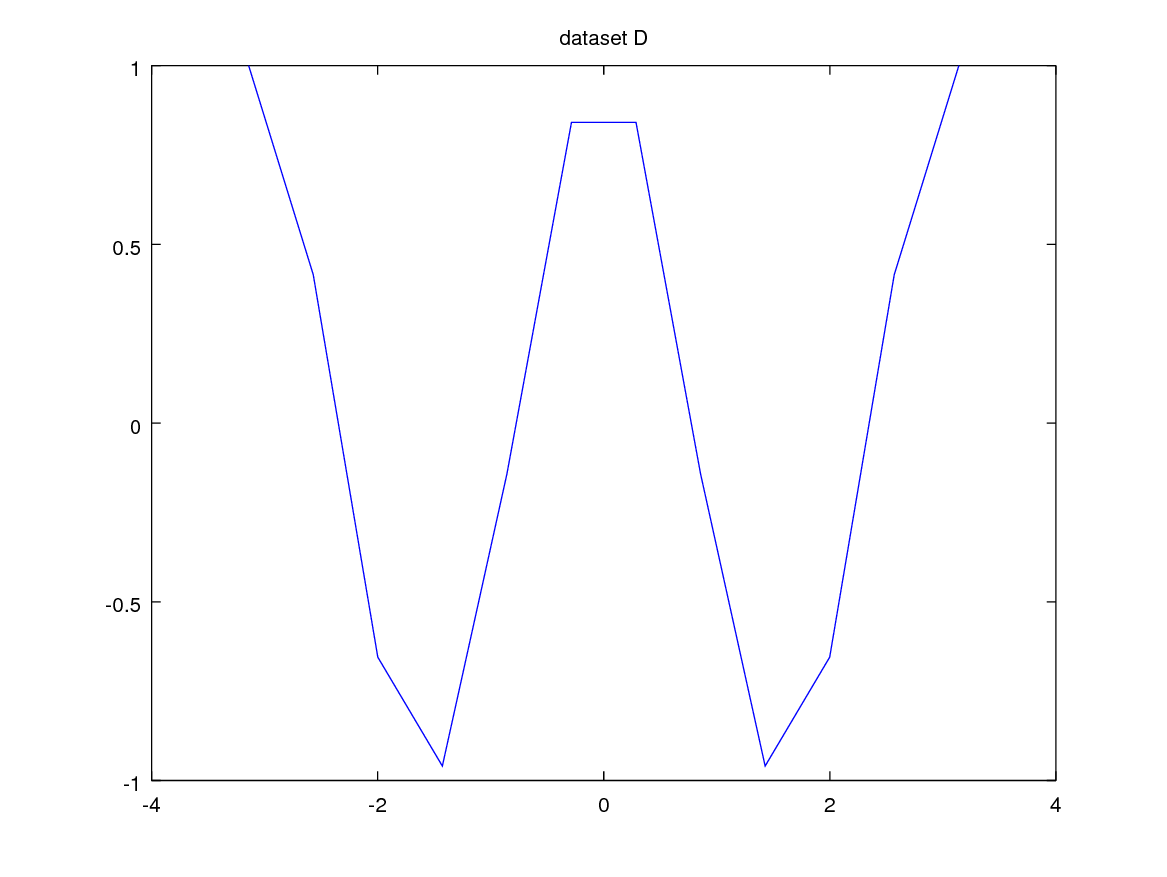
\includegraphics[width=.5\linewidth]{task4_hw1.png}
  \caption{dataset-D}
  \label{fig:dataset-D}
\end{figure}
the plot result is shown in Figure 1.
The matlab code for task 5 is shown below: 
\lstinputlisting{hw1_task5.m}

\section{Task 6}
the plots are shown with their corresponding value of dimension N: 
\begin{figure}[!htb]
   \begin{minipage}{0.48\textwidth}
     \centering
     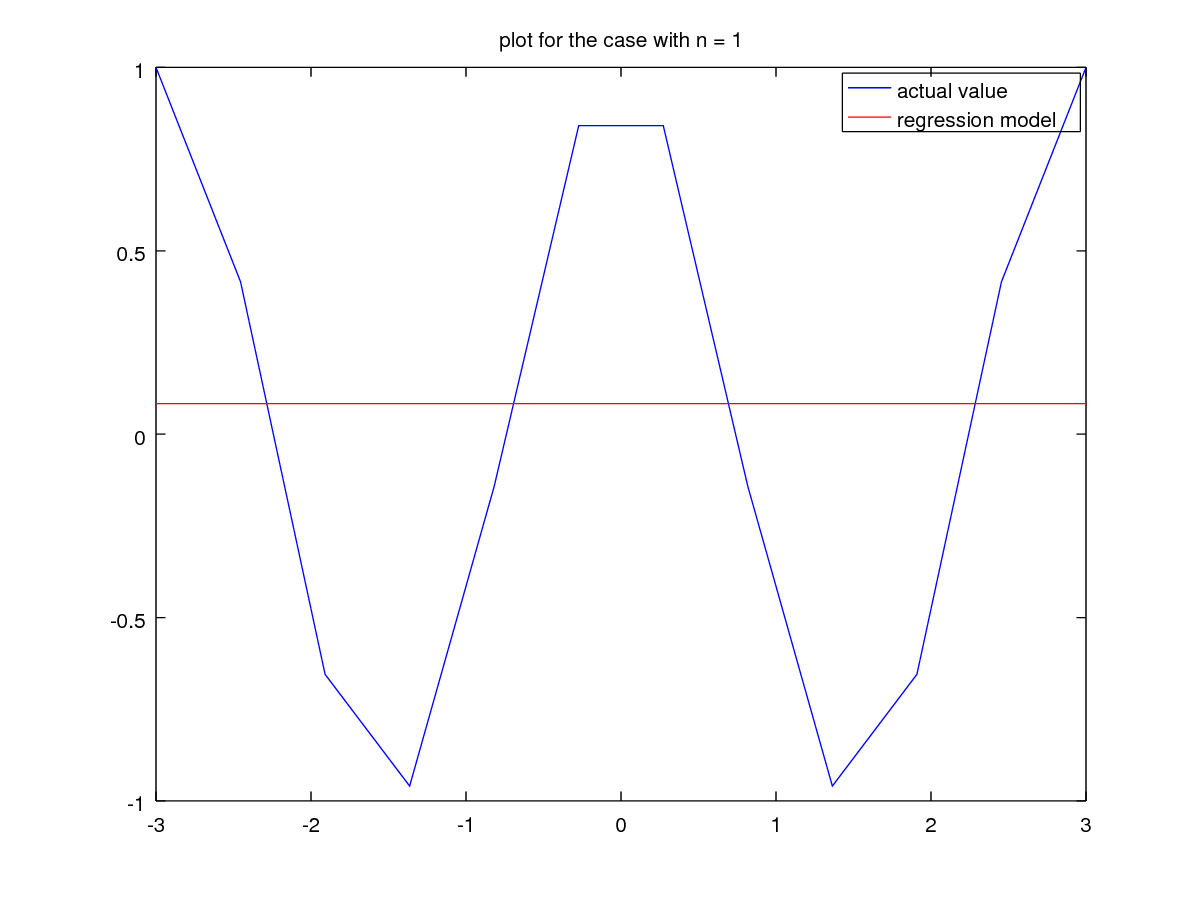
\includegraphics[width=.7\linewidth]{hw1_task6_fig1.png}
     \caption{M=1}\label{Fig:M=1}
   \end{minipage}\hfill
   \begin {minipage}{0.48\textwidth}
     \centering
     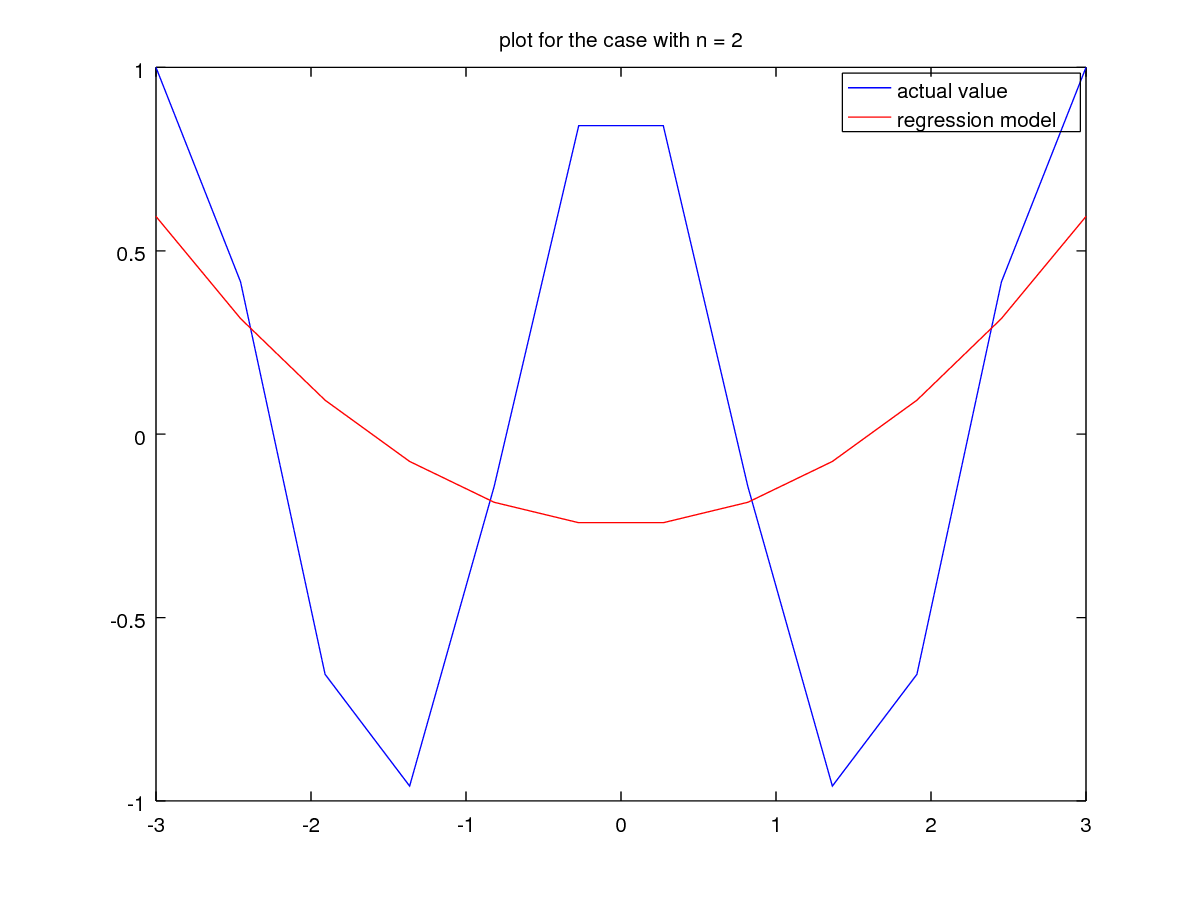
\includegraphics[width=.7\linewidth]{hw1_task6_fig2.png}
     \caption{M=2}\label{Fig:M=2}
   \end{minipage}\hfill 
   \begin{minipage}{0.48\textwidth}
     \centering
     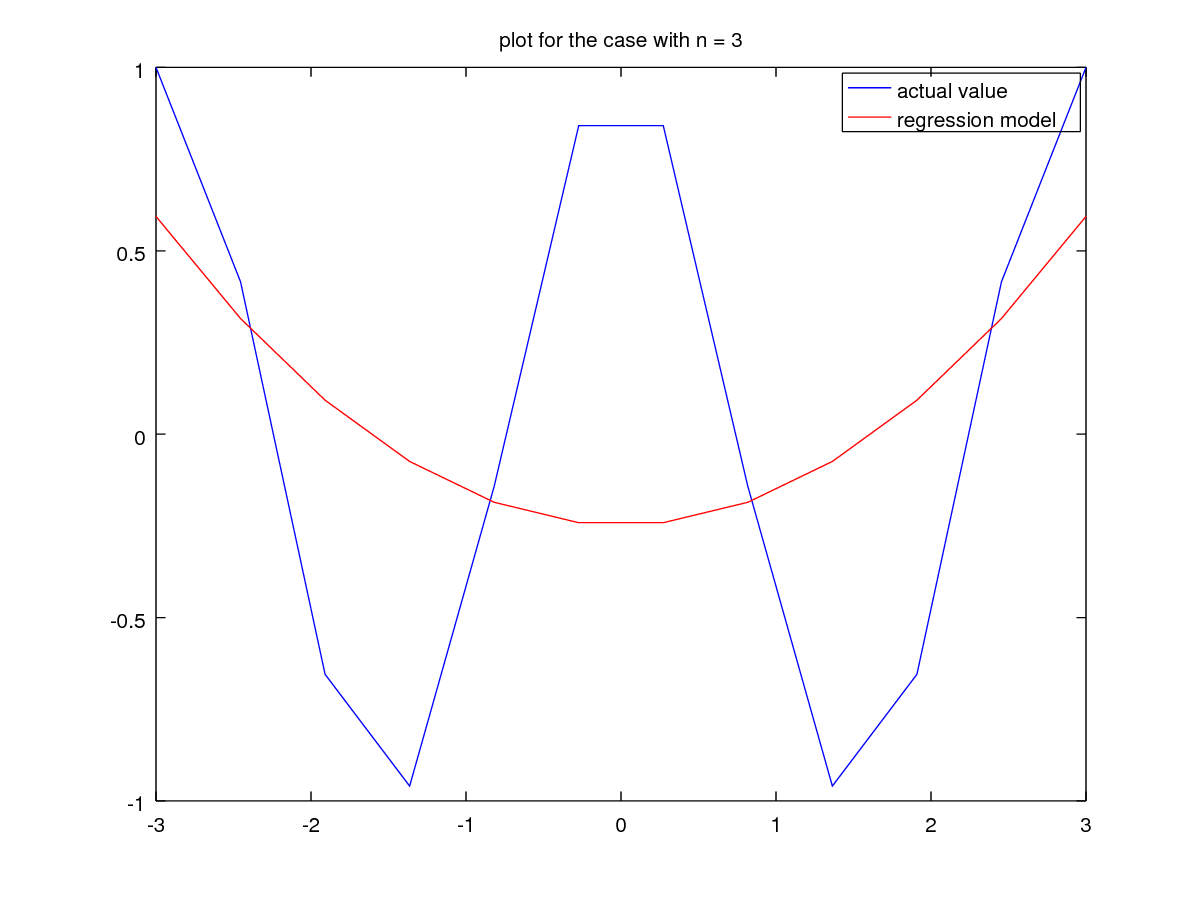
\includegraphics[width=.7\linewidth]{hw1_task6_fig3.png}
     \caption{M=3}\label{Fig:M=3}
   \end{minipage}\hfill
   \begin {minipage}{0.48\textwidth}
     \centering
     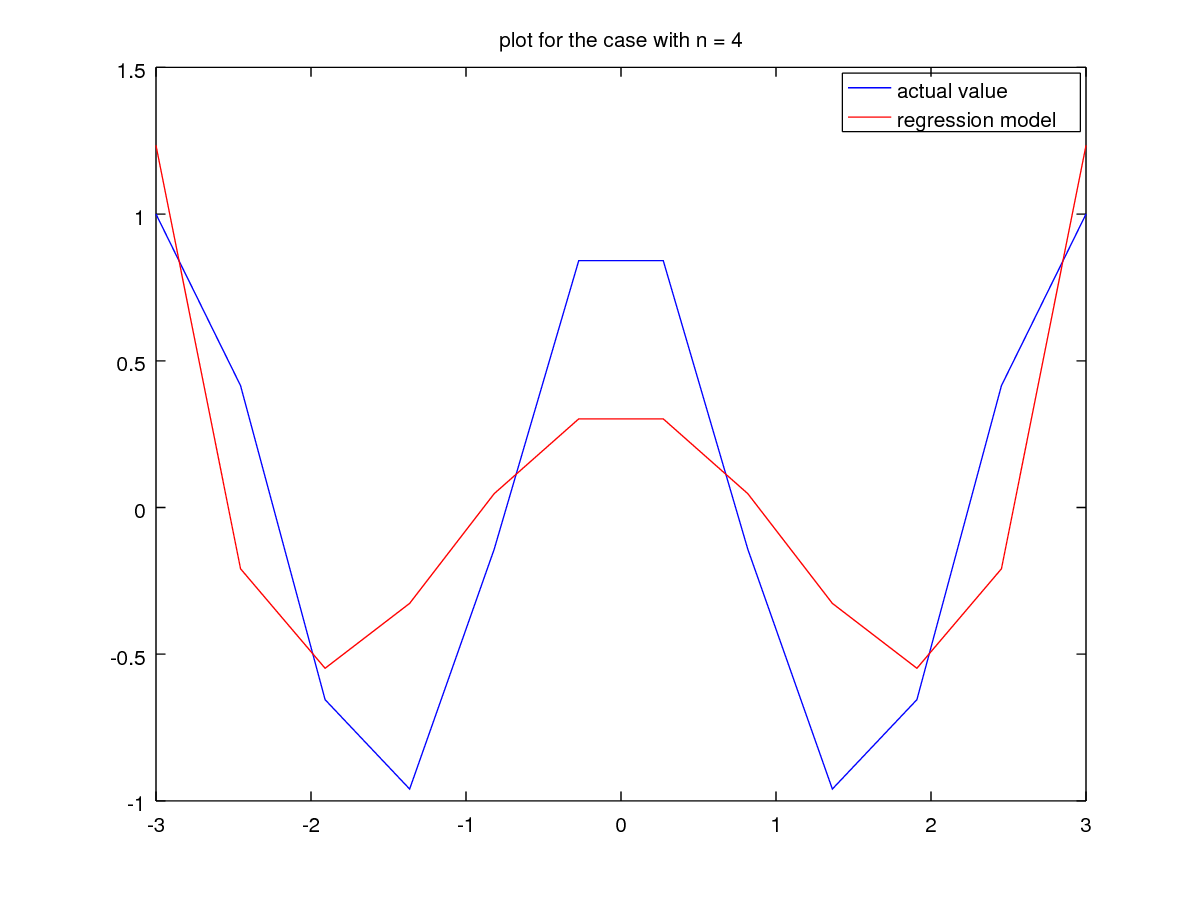
\includegraphics[width=.7\linewidth]{hw1_task6_fig4.png}
     \caption{M=4}\label{Fig:M=4}
   \end{minipage}\hfill
   \begin{minipage}{0.48\textwidth}
     \centering
     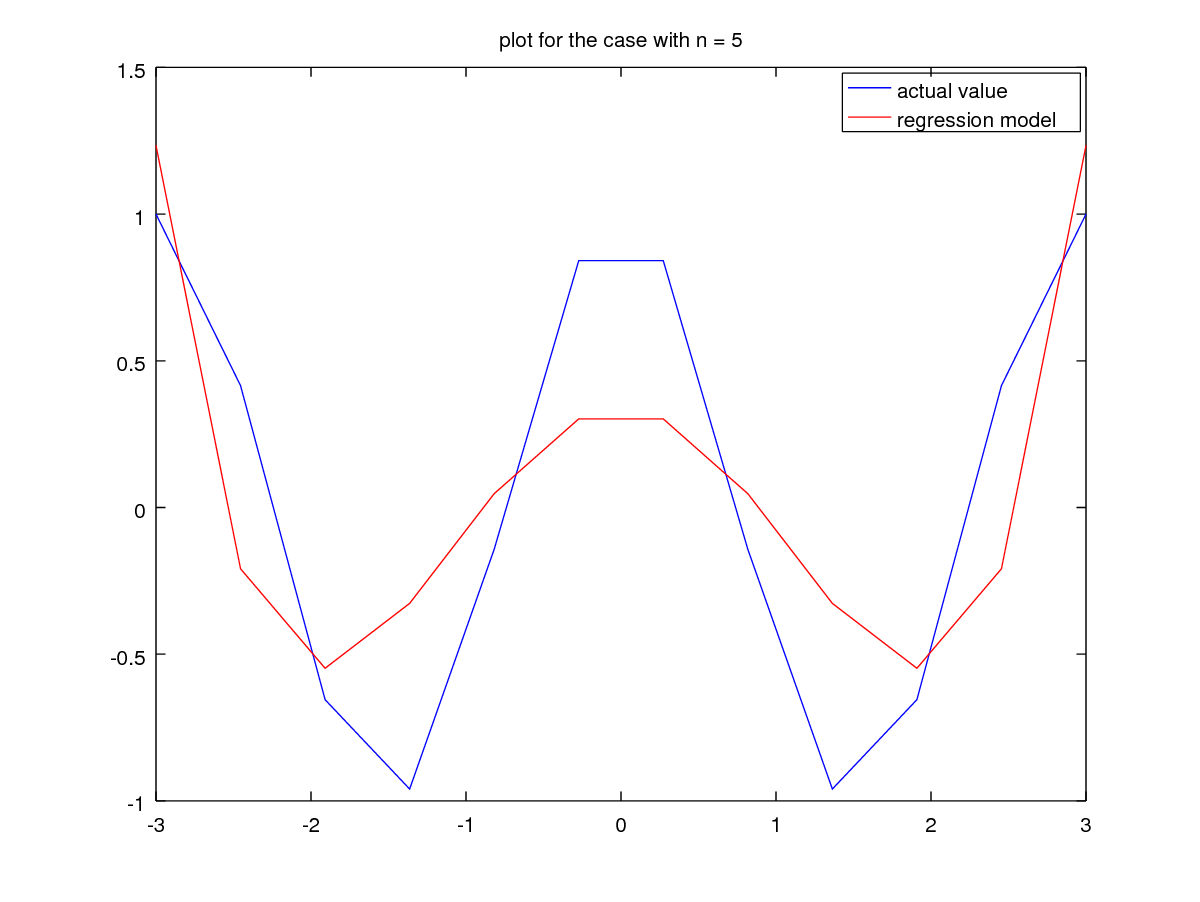
\includegraphics[width=.7\linewidth]{hw1_task6_fig5.png}
     \caption{M=5}\label{Fig:M=5}
   \end{minipage}\hfill
   \begin {minipage}{0.48\textwidth}
     \centering
     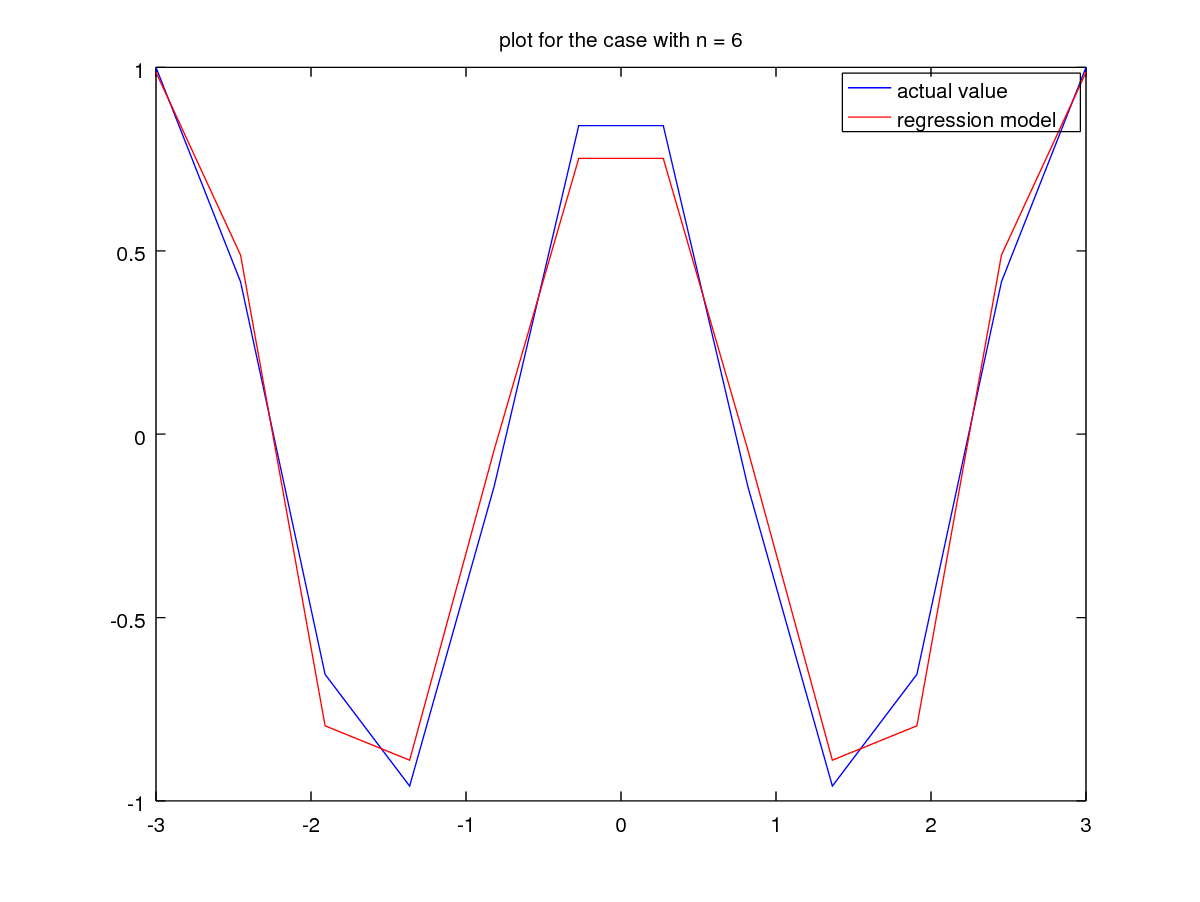
\includegraphics[width=.7\linewidth]{hw1_task6_fig6.png}
     \caption{M=6}\label{Fig:M=6}
   \end{minipage}\hfill
   \begin{minipage}{0.48\textwidth}
     \centering
     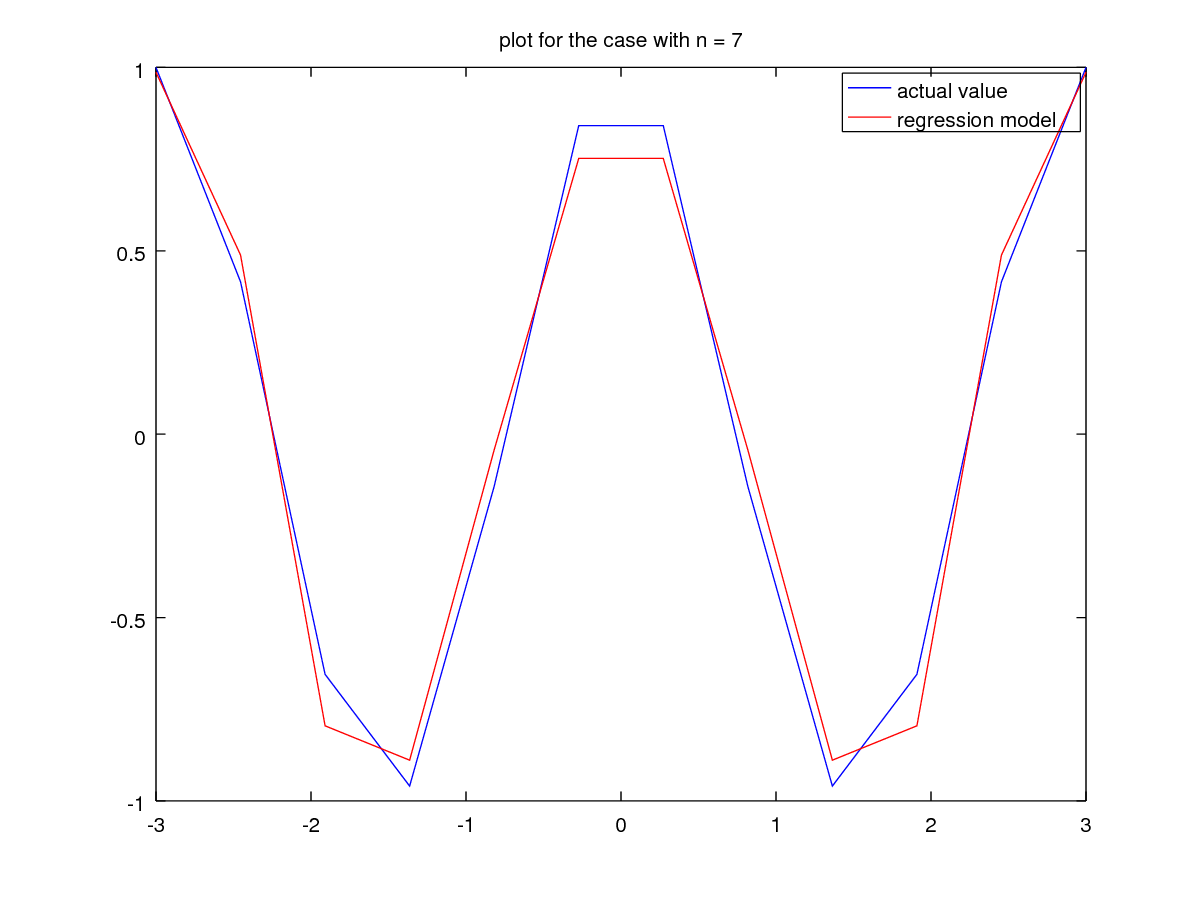
\includegraphics[width=.7\linewidth]{hw1_task6_fig7.png}
     \caption{M=7}\label{Fig:M=7}
   \end{minipage}\hfill
   \begin {minipage}{0.48\textwidth}
     \centering
     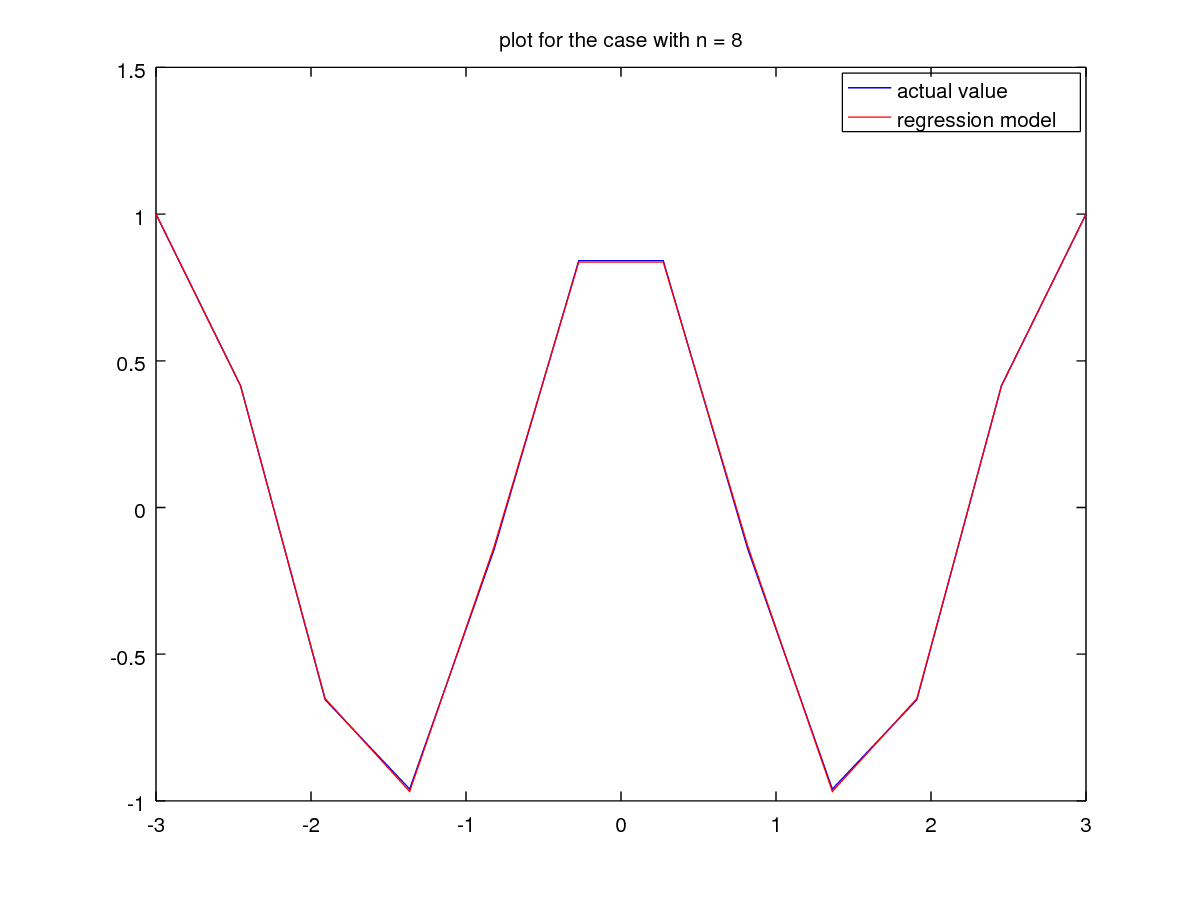
\includegraphics[width=.7\linewidth]{hw1_task6_fig8.png}
     \caption{M=8}\label{Fig:M=8}
   \end{minipage}
\end{figure} 
\begin{figure}[!htb]
   \begin{minipage}{0.48\textwidth}
     \centering
     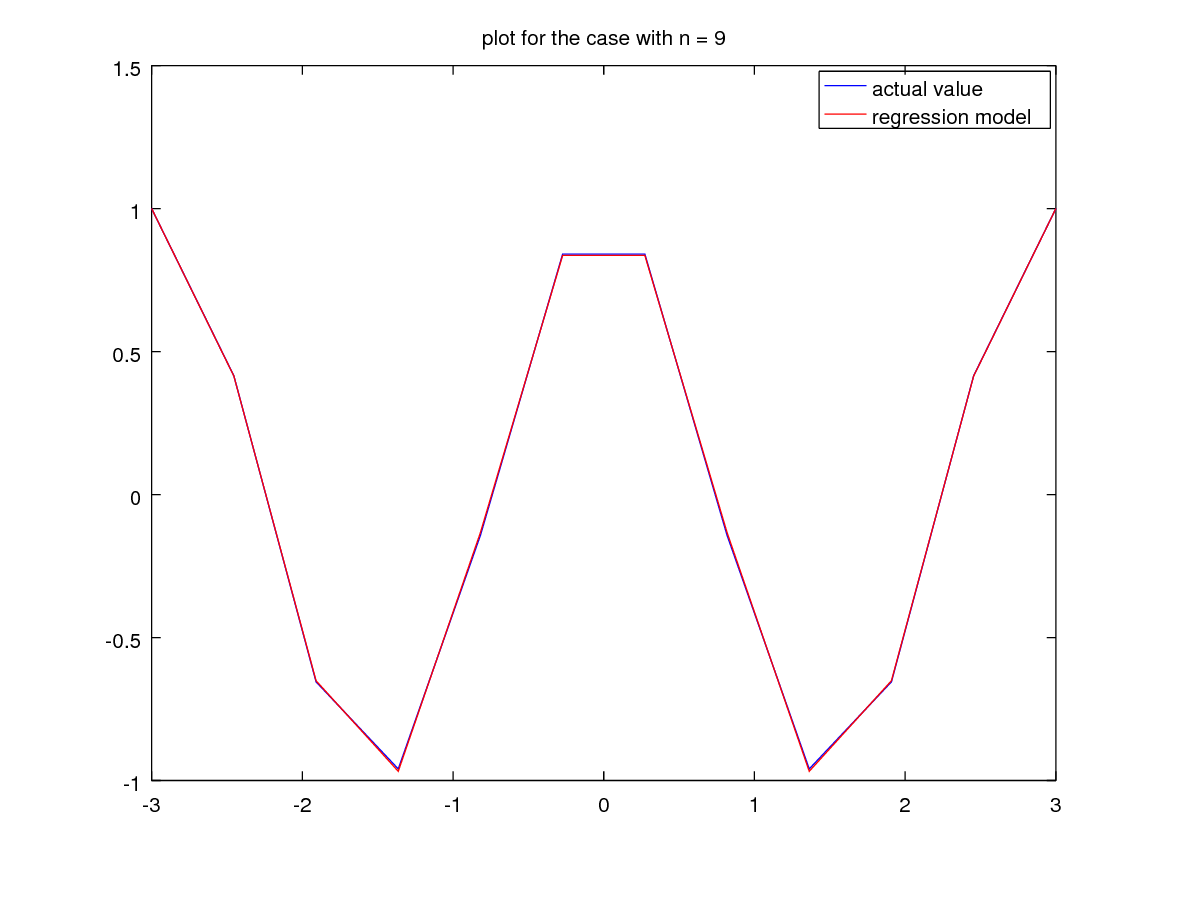
\includegraphics[width=.7\linewidth]{hw1_task6_fig9.png}
     \caption{M=9}\label{Fig:M=9}
   \end{minipage}\hfill
   \begin {minipage}{0.48\textwidth}
     \centering
     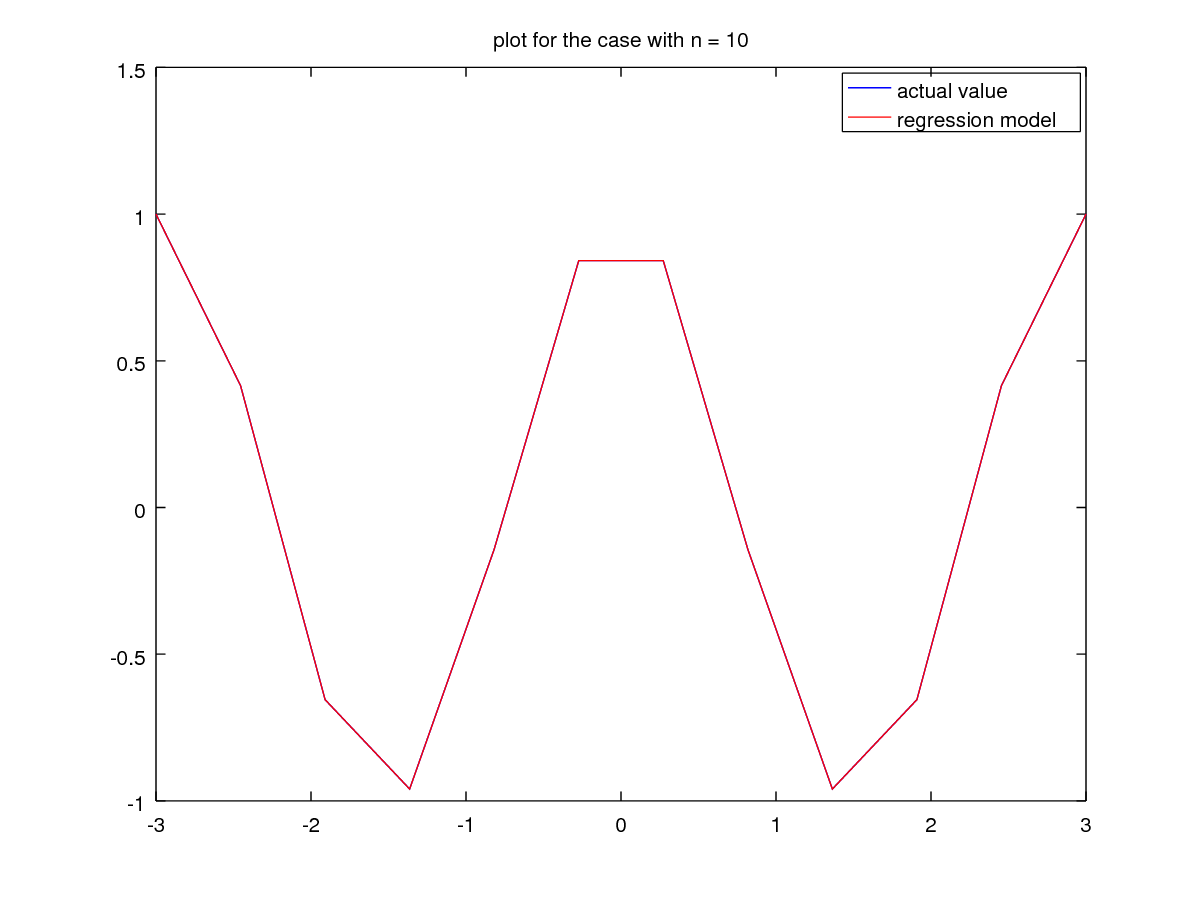
\includegraphics[width=.7\linewidth]{hw1_task6_fig10.png}
     \caption{M=10}\label{Fig:M=10}
   \end{minipage}\hfill
   \begin {minipage}{0.48\textwidth}
     \centering
     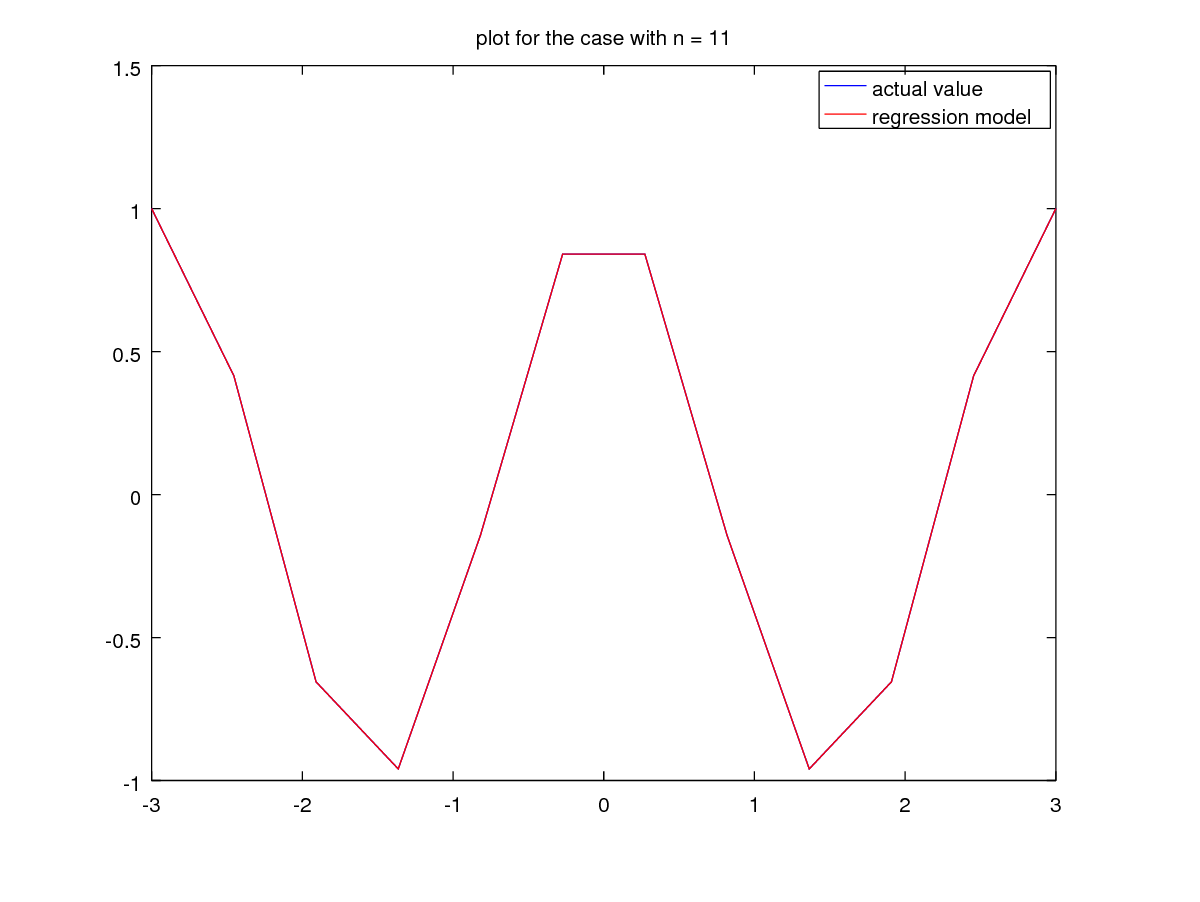
\includegraphics[width=.7\linewidth]{hw1_task6_fig11.png}
     \caption{M=11}\label{Fig:M=11}
   \end{minipage}
\end{figure}
From the plots, it is clear that approximation is more and more precise as higher dimension terms are introduced, from M = 9 and on, the plot is almost exactly the same as $f$.The matlab code is shown below: 
\lstinputlisting{hw1_task6.m}

\section{Task 7}
the random noise here is uniform random noise, the plot is shown in figure 13. 
\begin{figure}
  \centering 
  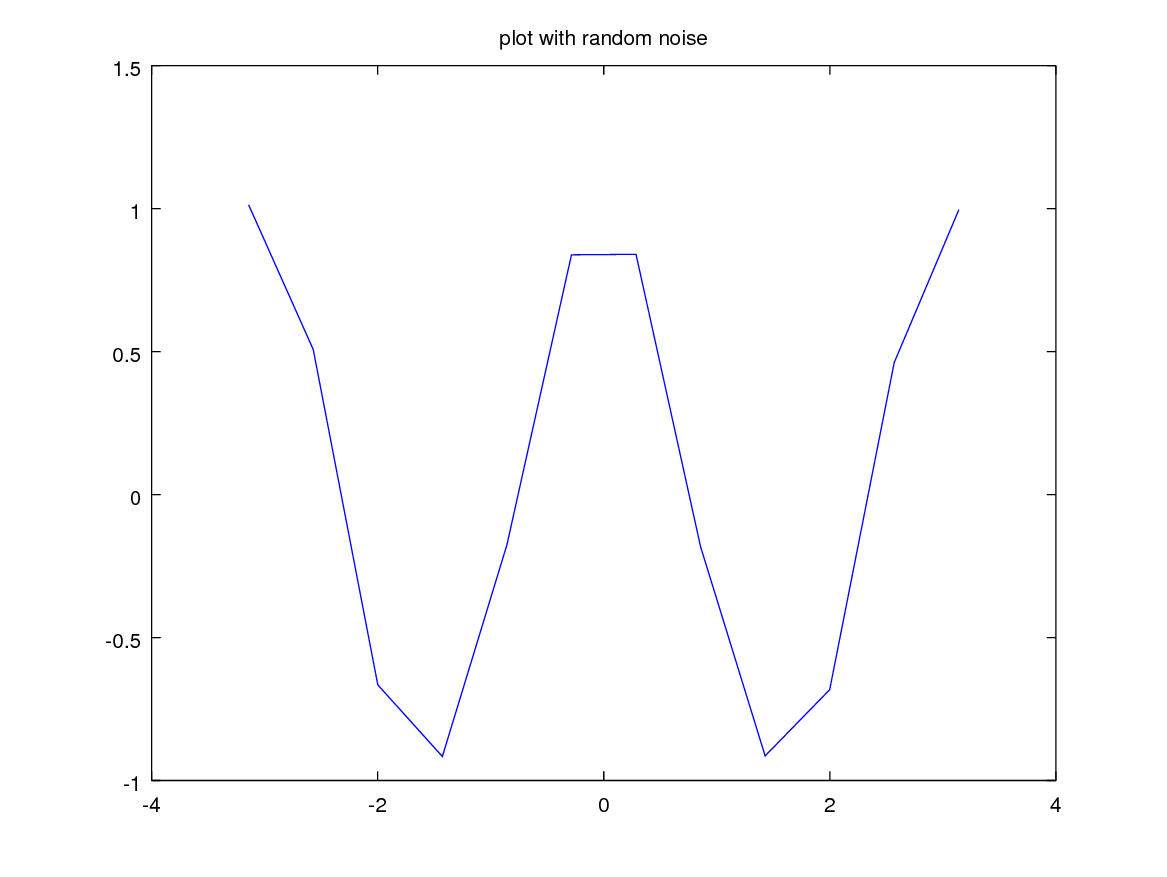
\includegraphics[width=.5\linewidth]{task7_hw1.png}
  \caption{random noise plot cos(x)}
  \label{fig:random noise plot cos(x)}
\end{figure}

\section{Task 8}
The comparison shows that with value of $M$ approach $N$, the result is generally more and more similar to $f$. However, it takes larger value of $M$ when random noise is introduced in the model.And in our case, when $M=10$, we have a better approximation than $M=11$ for function $f$. The result for $M = 11$ is shown in figure 14. 

\begin{figure}
  \centering 
  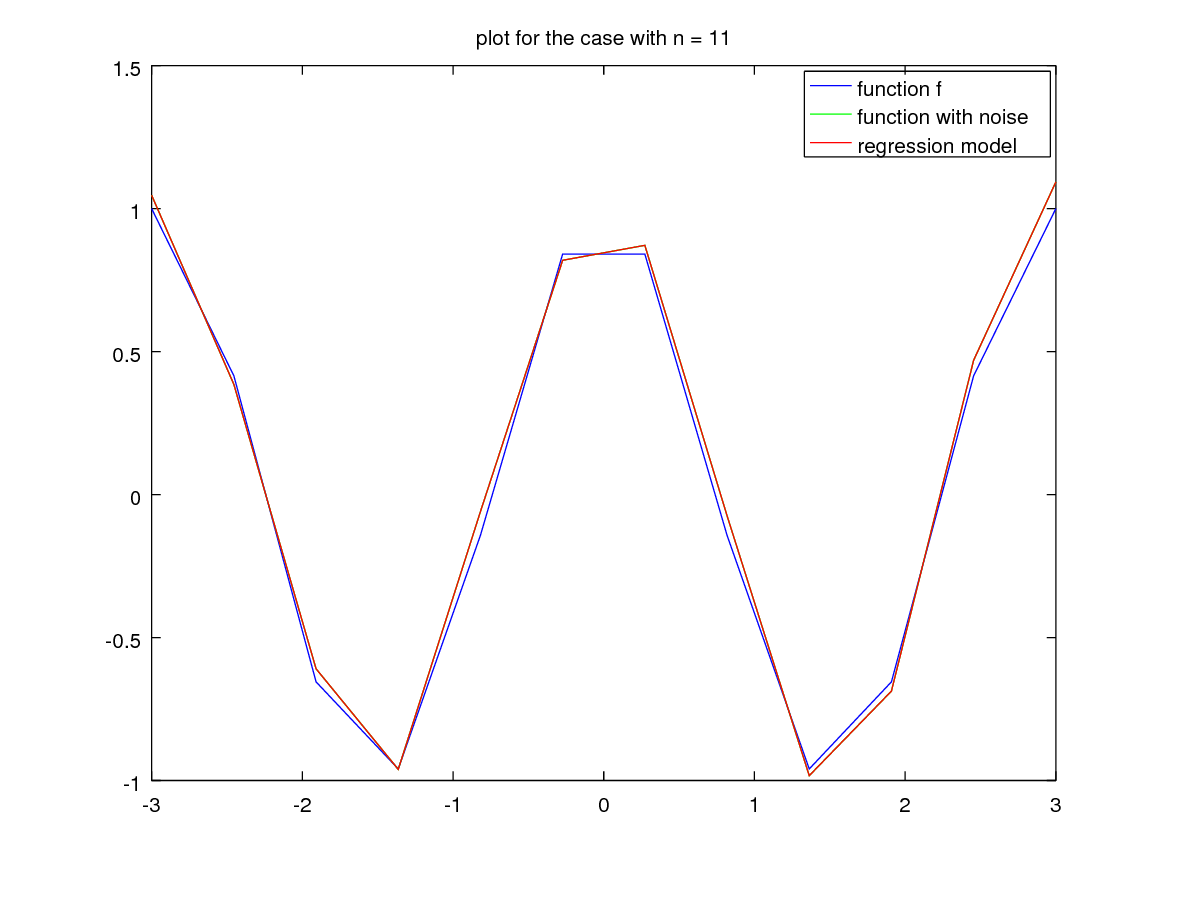
\includegraphics[width=.5\linewidth]{hw1_task8_fig11.png}
  \caption{M=11}
  \label{fig:M=11}
\end{figure}











\end{document}